% Options for packages loaded elsewhere
\PassOptionsToPackage{unicode}{hyperref}
\PassOptionsToPackage{hyphens}{url}
\PassOptionsToPackage{dvipsnames,svgnames,x11names}{xcolor}
%
\documentclass[
  letterpaper,
  DIV=11,
  numbers=noendperiod]{scrartcl}

\usepackage{amsmath,amssymb}
\usepackage{iftex}
\ifPDFTeX
  \usepackage[T1]{fontenc}
  \usepackage[utf8]{inputenc}
  \usepackage{textcomp} % provide euro and other symbols
\else % if luatex or xetex
  \usepackage{unicode-math}
  \defaultfontfeatures{Scale=MatchLowercase}
  \defaultfontfeatures[\rmfamily]{Ligatures=TeX,Scale=1}
\fi
\usepackage{lmodern}
\ifPDFTeX\else  
    % xetex/luatex font selection
\fi
% Use upquote if available, for straight quotes in verbatim environments
\IfFileExists{upquote.sty}{\usepackage{upquote}}{}
\IfFileExists{microtype.sty}{% use microtype if available
  \usepackage[]{microtype}
  \UseMicrotypeSet[protrusion]{basicmath} % disable protrusion for tt fonts
}{}
\makeatletter
\@ifundefined{KOMAClassName}{% if non-KOMA class
  \IfFileExists{parskip.sty}{%
    \usepackage{parskip}
  }{% else
    \setlength{\parindent}{0pt}
    \setlength{\parskip}{6pt plus 2pt minus 1pt}}
}{% if KOMA class
  \KOMAoptions{parskip=half}}
\makeatother
\usepackage{xcolor}
\setlength{\emergencystretch}{3em} % prevent overfull lines
\setcounter{secnumdepth}{-\maxdimen} % remove section numbering
% Make \paragraph and \subparagraph free-standing
\ifx\paragraph\undefined\else
  \let\oldparagraph\paragraph
  \renewcommand{\paragraph}[1]{\oldparagraph{#1}\mbox{}}
\fi
\ifx\subparagraph\undefined\else
  \let\oldsubparagraph\subparagraph
  \renewcommand{\subparagraph}[1]{\oldsubparagraph{#1}\mbox{}}
\fi


\providecommand{\tightlist}{%
  \setlength{\itemsep}{0pt}\setlength{\parskip}{0pt}}\usepackage{longtable,booktabs,array}
\usepackage{calc} % for calculating minipage widths
% Correct order of tables after \paragraph or \subparagraph
\usepackage{etoolbox}
\makeatletter
\patchcmd\longtable{\par}{\if@noskipsec\mbox{}\fi\par}{}{}
\makeatother
% Allow footnotes in longtable head/foot
\IfFileExists{footnotehyper.sty}{\usepackage{footnotehyper}}{\usepackage{footnote}}
\makesavenoteenv{longtable}
\usepackage{graphicx}
\makeatletter
\def\maxwidth{\ifdim\Gin@nat@width>\linewidth\linewidth\else\Gin@nat@width\fi}
\def\maxheight{\ifdim\Gin@nat@height>\textheight\textheight\else\Gin@nat@height\fi}
\makeatother
% Scale images if necessary, so that they will not overflow the page
% margins by default, and it is still possible to overwrite the defaults
% using explicit options in \includegraphics[width, height, ...]{}
\setkeys{Gin}{width=\maxwidth,height=\maxheight,keepaspectratio}
% Set default figure placement to htbp
\makeatletter
\def\fps@figure{htbp}
\makeatother

\usepackage{amssymb}
\usepackage{xcolor}
\usepackage{fancyhdr}
\pagestyle{fancy}
\fancyhead[L]{Project: Cap18 Validation \\ Task: Larsa Comparison}
\fancyhead[R]{Calculated by: CAM Date: 10/17/2024 \\Checked by:     Date:   /  /    }
\KOMAoption{captions}{tableheading}
\makeatletter
\@ifpackageloaded{caption}{}{\usepackage{caption}}
\AtBeginDocument{%
\ifdefined\contentsname
  \renewcommand*\contentsname{Table of contents}
\else
  \newcommand\contentsname{Table of contents}
\fi
\ifdefined\listfigurename
  \renewcommand*\listfigurename{List of Figures}
\else
  \newcommand\listfigurename{List of Figures}
\fi
\ifdefined\listtablename
  \renewcommand*\listtablename{List of Tables}
\else
  \newcommand\listtablename{List of Tables}
\fi
\ifdefined\figurename
  \renewcommand*\figurename{Figure}
\else
  \newcommand\figurename{Figure}
\fi
\ifdefined\tablename
  \renewcommand*\tablename{Table}
\else
  \newcommand\tablename{Table}
\fi
}
\@ifpackageloaded{float}{}{\usepackage{float}}
\floatstyle{ruled}
\@ifundefined{c@chapter}{\newfloat{codelisting}{h}{lop}}{\newfloat{codelisting}{h}{lop}[chapter]}
\floatname{codelisting}{Listing}
\newcommand*\listoflistings{\listof{codelisting}{List of Listings}}
\makeatother
\makeatletter
\makeatother
\makeatletter
\@ifpackageloaded{caption}{}{\usepackage{caption}}
\@ifpackageloaded{subcaption}{}{\usepackage{subcaption}}
\makeatother
\ifLuaTeX
  \usepackage{selnolig}  % disable illegal ligatures
\fi
\usepackage{bookmark}

\IfFileExists{xurl.sty}{\usepackage{xurl}}{} % add URL line breaks if available
\urlstyle{same} % disable monospaced font for URLs
\hypersetup{
  pdftitle={Cap18 Validation},
  colorlinks=true,
  linkcolor={blue},
  filecolor={Maroon},
  citecolor={Blue},
  urlcolor={Blue},
  pdfcreator={LaTeX via pandoc}}

\title{Cap18 Validation}
\author{}
\date{}

\begin{document}
\maketitle

\renewcommand*\contentsname{Table of contents}
{
\hypersetup{linkcolor=}
\setcounter{tocdepth}{3}
\tableofcontents
}
\newpage{}

\section{Example 2 - Six Column Bent (Back
Span)}\label{example-2---six-column-bent-back-span}

Example 2 was run for both Larsa and Cap18. Example 2 needed two
separate runs to effectively analyze for the backspan and the forward
span. This is the analysis of the back span part of the example. Below
is a short summary of the bent details.

Bent Details:

\begin{itemize}
\tightlist
\item
  9 Tx54 backspan girders
\item
  10 Tx54 forwardspan girders
\item
  78' wide bent
\item
  6 columns spaced at 14'
\end{itemize}

\subsection{Back Span}\label{back-span}

The figure below shows the beam spacing for the backspan girders. Since
Cap18 works in half-foot increments, the beam spacing was rounded to the
nearest increments. Both Cap18 and Larsa have the same spacing for the
beams.

\begin{figure}[H]

{\centering 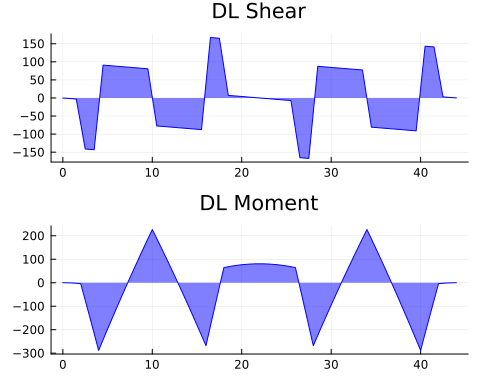
\includegraphics{03_six_col_bent_bk_files/mediabag/03_six_col_bent_bk_files/figure-pdf/cell-5-output-1.pdf}

}

\caption{Section View of Back Span}

\end{figure}%

\subsection{Forward Span}\label{forward-span}

The figure below shows the beam spacing for the forwardspan girders.

\begin{figure}[H]

{\centering 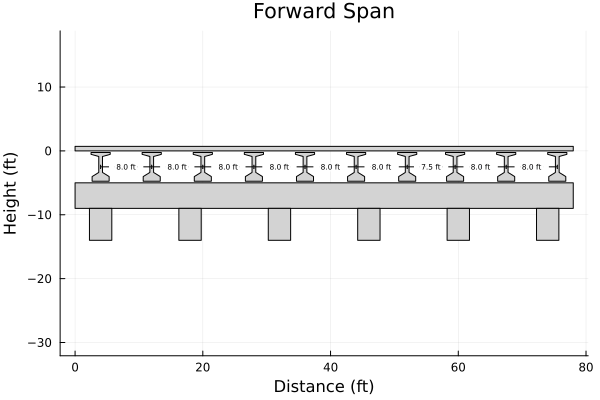
\includegraphics{03_six_col_bent_bk_files/mediabag/03_six_col_bent_bk_files/figure-pdf/cell-6-output-1.pdf}

}

\caption{Section View of Forward Span}

\end{figure}%

\newpage{}

\section{Cap 18}\label{cap-18}

A Cap18 input file was created and ran for the above bent. The output
file was then parsed for the dead load, working stress, and load factor
cases. The summary of the findings are discussed below.

\subsection{SRV}\label{srv}

\subsubsection{Dead Load Results (SRV)}\label{dead-load-results-srv}

The dead load results were plotted on top of the bent to get a better
visual understanding of the results. Based on the DL shear and moment
diagrams below, the Cap18 results look to align well with the bent.
Sharp changes in shear happen in areas with either a column or a beam,
and negative moments are maximized over the columns. This indicates to
some degree that the expected behavior of the stresses within the cap is
being captured by the Cap18 program. A more detailed comparison with
Larsa results will help determine if the magnitudes of these stresses
are correct.

\begin{figure}[H]

{\centering 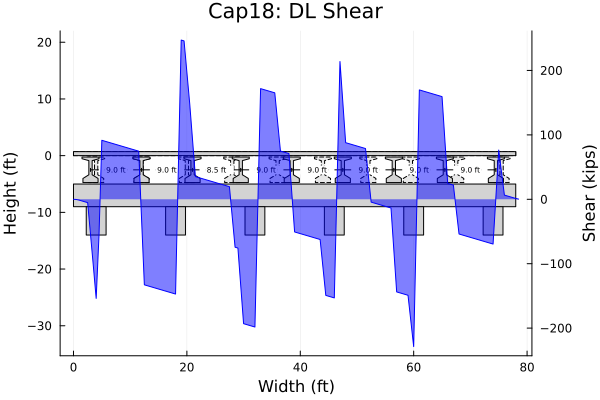
\includegraphics{03_six_col_bent_bk_files/mediabag/03_six_col_bent_bk_files/figure-pdf/cell-8-output-1.pdf}

}

\caption{Cap18: DL Shear Diagram}

\end{figure}%

\begin{figure}[H]

{\centering 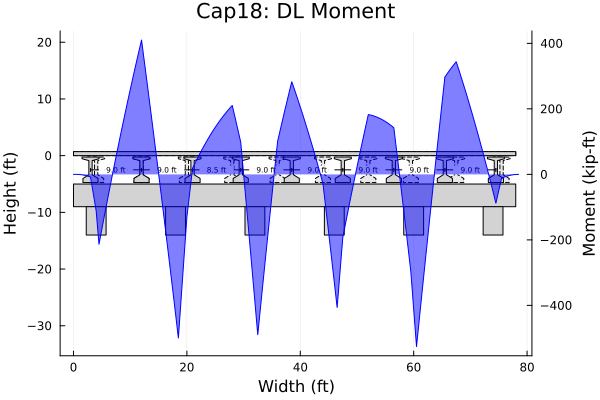
\includegraphics{03_six_col_bent_bk_files/mediabag/03_six_col_bent_bk_files/figure-pdf/cell-9-output-1.pdf}

}

\caption{Cap18: DL Moment Diagram}

\end{figure}%

\newpage{}

\subsubsection{Envelopes of Maximum Values
(SRV)}\label{envelopes-of-maximum-values-srv}

The working stress results were plotted on top of the bent to get a
better visual understanding of the results. The results can be seen in
the figures below. These stresses follow the same expected behavoir as
the DL stresses. Further comparison with Larsa is needed.

\begin{figure}[H]

{\centering 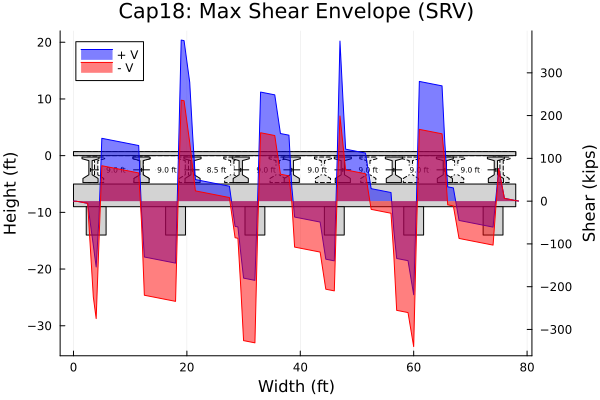
\includegraphics{03_six_col_bent_bk_files/mediabag/03_six_col_bent_bk_files/figure-pdf/cell-10-output-1.pdf}

}

\caption{Cap18: Service Shear Envelope Diagram}

\end{figure}%

\begin{figure}[H]

{\centering 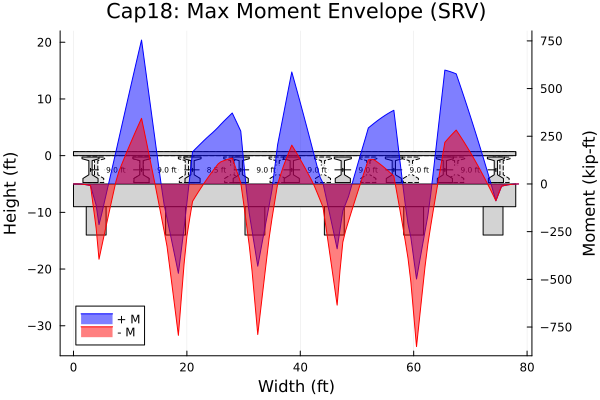
\includegraphics{03_six_col_bent_bk_files/mediabag/03_six_col_bent_bk_files/figure-pdf/cell-11-output-1.pdf}

}

\caption{Cap18: Service Moment Envelope Diagram}

\end{figure}%

\subsubsection{Maximum Support Reactions
(SRV)}\label{maximum-support-reactions-srv}

The maximum and minimum support reactions for the working stress case
are listed in the table below.

\begin{longtable}[]{@{}rrrr@{}}
\caption{Cap18: Service Reactions}\tabularnewline
\toprule\noalign{}
Station & Distance & Max Reactions & Min Reactions \\
\midrule\noalign{}
\endfirsthead
\toprule\noalign{}
Station & Distance & Max Reactions & Min Reactions \\
\midrule\noalign{}
\endhead
\bottomrule\noalign{}
\endlastfoot
9 & 4.5 ft & 465.3 kip & 288.4 kip \\
37 & 18.5 ft & 613.5 kip & 383.5 kip \\
65 & 32.5 ft & 587.7 kip & 347.7 kip \\
93 & 46.5 ft & 585.6 kip & 341.3 kip \\
121 & 60.5 ft & 622.6 kip & 389.2 kip \\
149 & 74.5 ft & 427.3 kip & 267.5 kip \\
\end{longtable}

\newpage{}

\subsection{STR}\label{str}

\subsubsection{Envelopes of Maximum Values
(STR)}\label{envelopes-of-maximum-values-str}

The load factor results were plotted on top of the bent to get a better
visual understanding of the results. The results can be seen in the
figures below. These stresses follow the same expected behavoir as the
DL stresses. Further comparison with Larsa is needed.

\begin{figure}[H]

{\centering 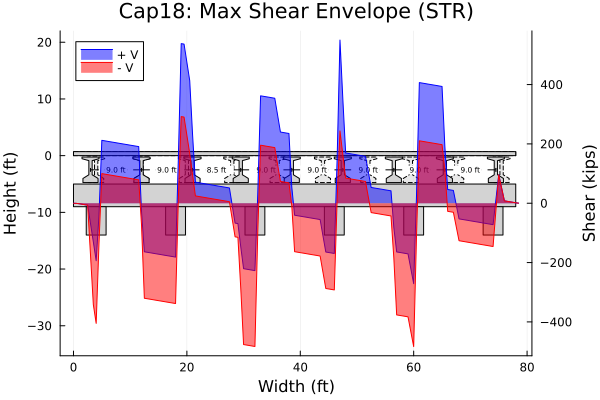
\includegraphics{03_six_col_bent_bk_files/mediabag/03_six_col_bent_bk_files/figure-pdf/cell-13-output-1.pdf}

}

\caption{Cap18: Strength Shear Envelope Diagram}

\end{figure}%

\begin{figure}[H]

{\centering 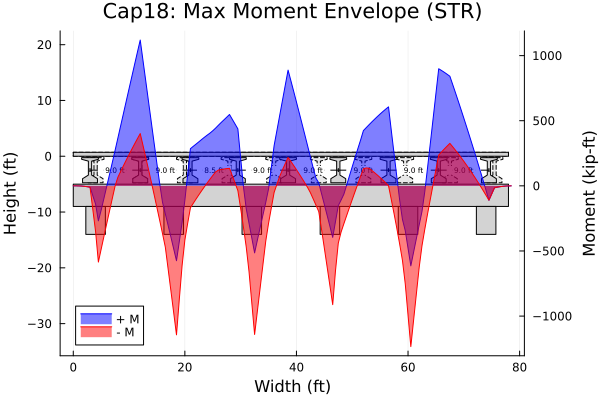
\includegraphics{03_six_col_bent_bk_files/mediabag/03_six_col_bent_bk_files/figure-pdf/cell-14-output-1.pdf}

}

\caption{Cap18: Strength Moment Envelope Diagram}

\end{figure}%

\subsubsection{Maximum Support Reactions
(STR)}\label{maximum-support-reactions-str}

The maximum and minimum support reactions for the load factor case are
listed in the table below.

\begin{table}
\caption{Cap18: Strength Reactions}\tabularnewline

\centering
\begin{tabular}{r|cccc}
    & sta & dist & max\_reaction & min\_reaction\\
    \hline
    & Int64 & Float64 & Float64 & Float64\\
    \hline
    1 & 9 & 4.5 & 668.3 & 358.8 \\
    2 & 37 & 18.5 & 879.4 & 476.8 \\
    3 & 65 & 32.5 & 846.0 & 426.0 \\
    4 & 93 & 46.5 & 843.7 & 416.3 \\
    5 & 121 & 60.5 & 893.2 & 484.7 \\
    6 & 149 & 74.5 & 612.1 & 332.4 \\
\end{tabular}
\end{table}

\newpage{}

\section{Larsa Results}\label{larsa-results}

A Larsa model was created and ran for the above bent. The loads were
extracted for the dead load, working stress, and load factor cases. The
summary of the findings are discussed below.

\subsection{SRV}\label{srv-1}

\subsubsection{Dead Load Results (SRV)}\label{dead-load-results-srv-1}

The dead load results were plotted on top of the bent to get a better
visual understanding of the results. Based on the DL shear and moment
diagrams below, the Larsa results look to align well with the bent. A
more detailed comparison with the Cap18 results will help determine if
the magnitudes of the stresses calculated from the Cap18 program are
correct.

\begin{figure}[H]

{\centering \includegraphics{03_six_col_bent_bk_files/mediabag/03_six_col_bent_bk_files/figure-pdf/cell-17-output-1.pdf}

}

\caption{LARSA: DL Shear Diagram}

\end{figure}%

\begin{figure}[H]

{\centering \includegraphics{03_six_col_bent_bk_files/mediabag/03_six_col_bent_bk_files/figure-pdf/cell-18-output-1.pdf}

}

\caption{LARSA: DL Moment Diagram}

\end{figure}%

\newpage{}

\subsubsection{Envelopes of Maximum Values
(SRV)}\label{envelopes-of-maximum-values-srv-1}

The working stress results were plotted on top of the bent to get a
better visual understanding of the results. The results can be seen in
the figures below. These stresses follow the same expected behavoir as
the DL stresses. Further comparison with Cap18 is needed.

\begin{figure}[H]

{\centering 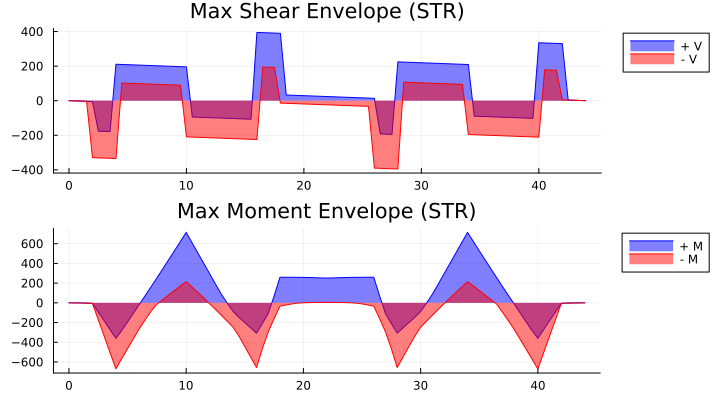
\includegraphics{03_six_col_bent_bk_files/mediabag/03_six_col_bent_bk_files/figure-pdf/cell-19-output-1.pdf}

}

\caption{LARSA: Service Shear Envelope Diagram}

\end{figure}%

\begin{figure}[H]

{\centering 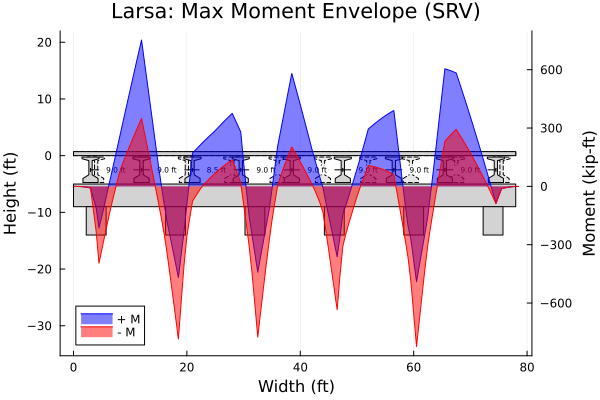
\includegraphics{03_six_col_bent_bk_files/mediabag/03_six_col_bent_bk_files/figure-pdf/cell-20-output-1.pdf}

}

\caption{LARSA: Service Moment Envelope Diagram}

\end{figure}%

\subsubsection{Maximum Support Reactions
(SRV)}\label{maximum-support-reactions-srv-1}

The maximum and minimum support reactions for the working stress case
are listed in the table below.

\begin{longtable}[]{@{}rrrr@{}}
\caption{LARSA: Service Reactions}\tabularnewline
\toprule\noalign{}
Station & Distance & Max Reactions & Min Reactions \\
\midrule\noalign{}
\endfirsthead
\toprule\noalign{}
Station & Distance & Max Reactions & Min Reactions \\
\midrule\noalign{}
\endhead
\bottomrule\noalign{}
\endlastfoot
9 & 4.5 ft & 465.86 kip & 289.142 kip \\
37 & 18.5 ft & 616.513 kip & 384.262 kip \\
65 & 32.5 ft & 585.038 kip & 350.561 kip \\
93 & 46.5 ft & 586.099 kip & 347.547 kip \\
121 & 60.5 ft & 617.082 kip & 387.892 kip \\
149 & 74.5 ft & 437.109 kip & 269.025 kip \\
\end{longtable}

\newpage{}

\subsection{STR}\label{str-1}

\subsubsection{Envelopes of Maximum Values
(STR)}\label{envelopes-of-maximum-values-str-1}

The load factor results were plotted on top of the bent to get a better
visual understanding of the results. The results can be seen in the
figures below. These stresses follow the same expected behavoir as the
DL stresses. Further comparison with Cap18 is needed.

\begin{figure}[H]

{\centering 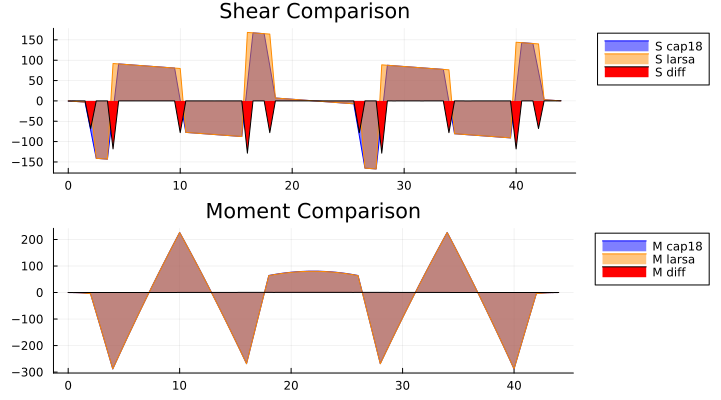
\includegraphics{03_six_col_bent_bk_files/mediabag/03_six_col_bent_bk_files/figure-pdf/cell-22-output-1.pdf}

}

\caption{LARSA: Strength Shear Envelope Diagram}

\end{figure}%

\begin{figure}[H]

{\centering 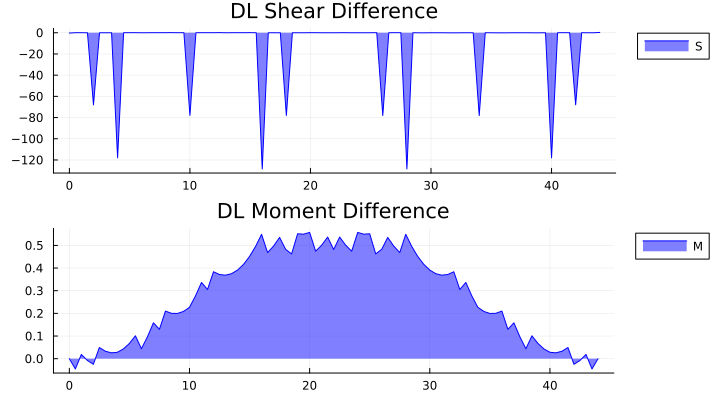
\includegraphics{03_six_col_bent_bk_files/mediabag/03_six_col_bent_bk_files/figure-pdf/cell-23-output-1.pdf}

}

\caption{LARSA: Strength Moment Envelope Diagram}

\end{figure}%

\subsubsection{Maximum Support Reactions
(STR)}\label{maximum-support-reactions-str-1}

The maximum and minimum support reactions for the load factor case are
listed in the table below.

\begin{longtable}[]{@{}rrrr@{}}
\caption{LARSA: Strength Reactions}\tabularnewline
\toprule\noalign{}
Station & Distance & Max Reactions & Min Reactions \\
\midrule\noalign{}
\endfirsthead
\toprule\noalign{}
Station & Distance & Max Reactions & Min Reactions \\
\midrule\noalign{}
\endhead
\bottomrule\noalign{}
\endlastfoot
9 & 4.5 ft & 669.094 kip & 359.836 kip \\
37 & 18.5 ft & 848.741 kip & 478.514 kip \\
65 & 32.5 ft & 809.339 kip & 431.215 kip \\
93 & 46.5 ft & 807.774 kip & 426.186 kip \\
121 & 60.5 ft & 852.34 kip & 483.67 kip \\
149 & 74.5 ft & 628.815 kip & 334.667 kip \\
\end{longtable}

\newpage{}

\section{Comparison}\label{comparison}

Below is a comparison of the Cap18 and Larsa results. Stresses were
found to be fairly similar between the different programs. The main
differences are in the shear stresses. Cap18 seems to have a more
gradual change in shear compared to Larsa. This is most likely due to
the way Cap18 defines the point loads in the program. This gradual vs
more sharp change in shear does not seem to affect the moment diagram in
a significant way. Moment diagram stresses do show some differences and
will be discussed in more detail below.

\textbf{Important Plot Information}\\
The comparison plots for the shear and moment diagrams are shown below
for all the different load cases. The Cap18 results are shown in a blue
line and the larsa results are shown in a red line. The red line will
only really be visible when the larsa results are greater in magnitude
than the cap18 results. The thickness of the red or blue line shows how
much greater in magnitdue the respective result was. The absolute
difference between larsa and cap18 is show in yellow. Any positive
yellow results indicate that larsa was greater in magnitude. Data labels
are also visible for the moment diagrams at the local extrema. Text in
blue indicates that Cap18 was greater in magnitude, while red text
indicates larsa results were greater in magnitude.

\newpage{}

\subsection{SRV}\label{srv-2}

\subsubsection{Dead Load Results (SRV)}\label{dead-load-results-srv-2}

The figures below compare the DL results between the two programs. The
areas in red highlight where larsa results were greater in magnitude
than the cap18 results. There are some visible red areas in the shear
diagram. However, these can be explained by the difference in point load
modeling between the two programs. The maximum values are shown to be
very similar. In areas of maximum moment and shears, the results are
within 3\%.

\begin{figure}[H]

{\centering 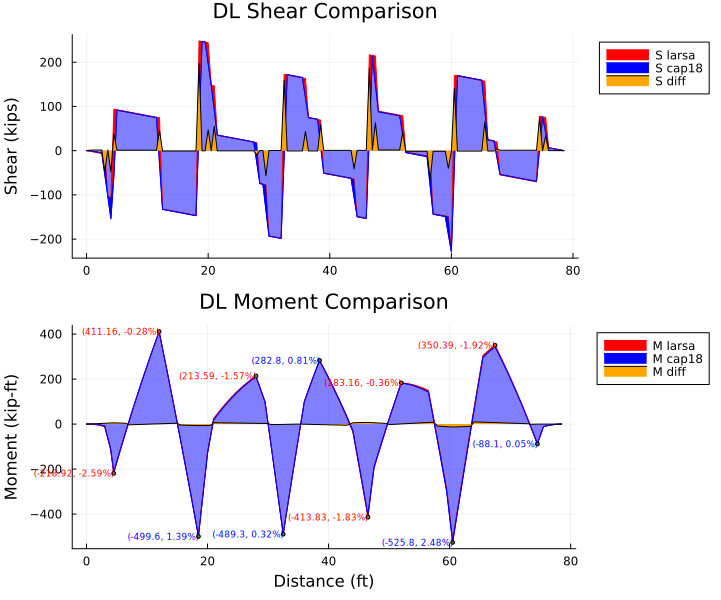
\includegraphics{03_six_col_bent_bk_files/mediabag/03_six_col_bent_bk_files/figure-pdf/cell-25-output-1.pdf}

}

\caption{Comparison: DL Shear and Moment Diagrams}

\end{figure}%

\begin{figure}[H]

{\centering 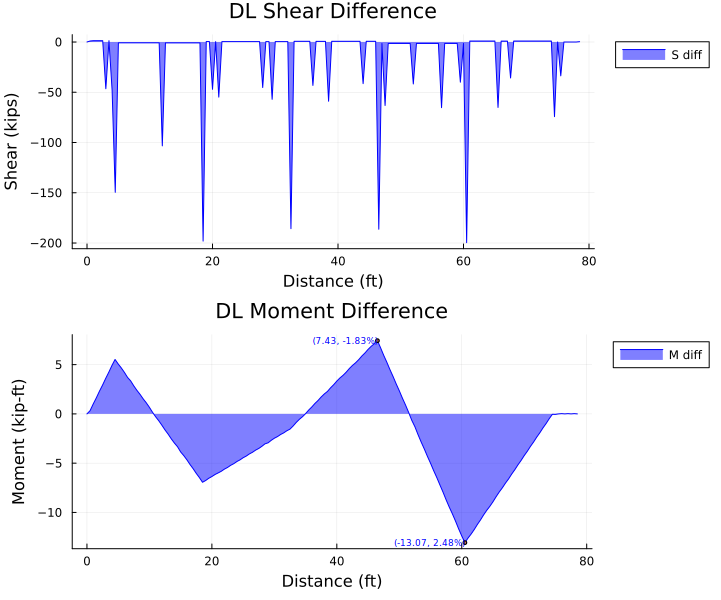
\includegraphics{03_six_col_bent_bk_files/mediabag/03_six_col_bent_bk_files/figure-pdf/cell-26-output-1.pdf}

}

\caption{Comparison: DL Shear and Moment Difference}

\end{figure}%

\newpage{}

\subsubsection{Envelopes of Maximum Values
(SRV)}\label{envelopes-of-maximum-values-srv-2}

\paragraph{Maximum Envelope
Comparison}\label{maximum-envelope-comparison}

The figures below compare the working stress results for the maximum
stress envelope between the two programs. The areas in red highlight
where larsa results were greater in magnitude than the cap18 results.
There are some visible red areas in the shear diagram. However, these
can be explained by the difference in point load modeling between the
two programs. The maximum values are shown to be very similar. In areas
of maximum moment and shears, the results are within 3\%.

\begin{figure}[H]

{\centering 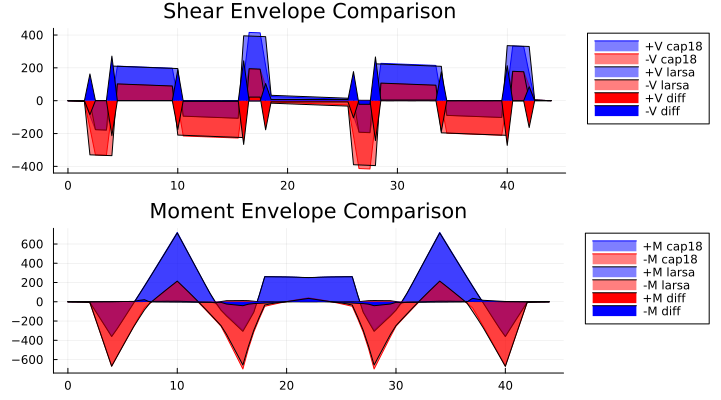
\includegraphics{03_six_col_bent_bk_files/mediabag/03_six_col_bent_bk_files/figure-pdf/cell-27-output-1.pdf}

}

\caption{Comparison: Service Shear and Moment Max Envelope Diagrams}

\end{figure}%

\begin{figure}[H]

{\centering 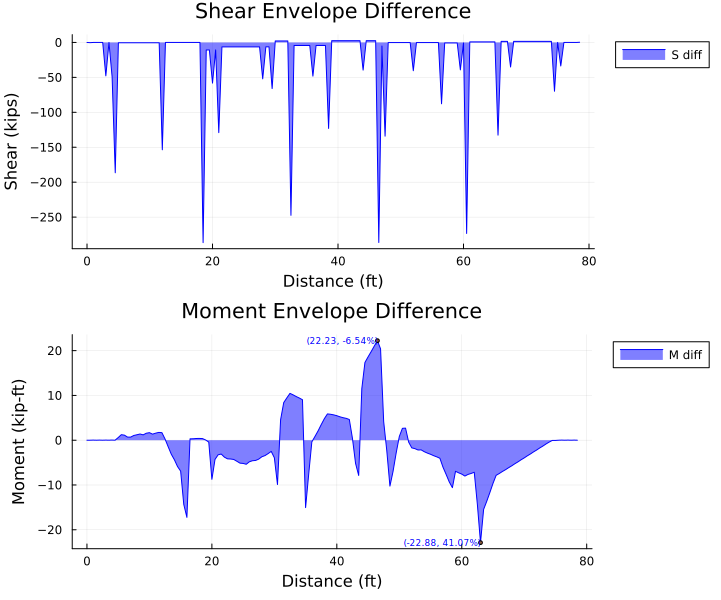
\includegraphics{03_six_col_bent_bk_files/mediabag/03_six_col_bent_bk_files/figure-pdf/cell-28-output-1.pdf}

}

\caption{Comparison: Service Shear and Moment Max Envelope Difference}

\end{figure}%

\newpage{}

\paragraph{Minimum Envelope
Comparison}\label{minimum-envelope-comparison}

The figures below compare the working stress results for the minimum
stress envelope between the two programs. The areas in red (not the
light red areas) highlight where larsa results were greater in magnitude
than the cap18 results. There are some visible red areas in the shear
diagram. However, these can be explained by the difference in point load
modeling between the two programs. . In areas of maximum moment and
shears, the results are within 4\%.

\begin{figure}[H]

{\centering 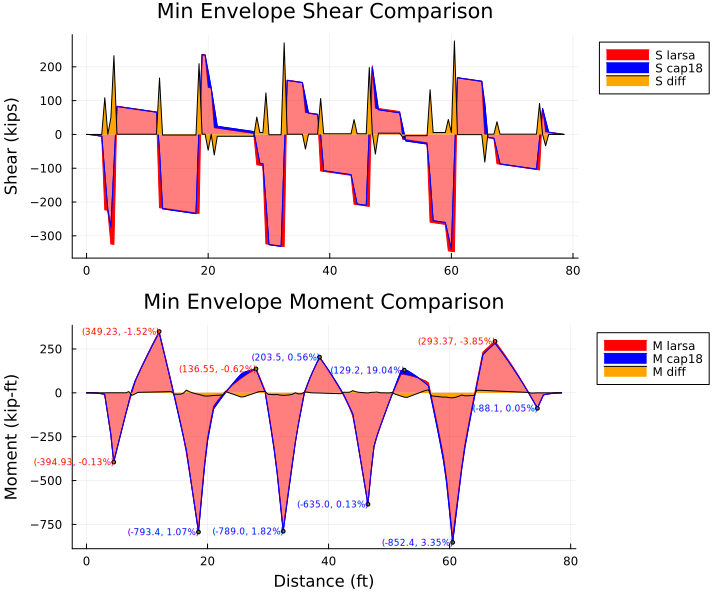
\includegraphics{03_six_col_bent_bk_files/mediabag/03_six_col_bent_bk_files/figure-pdf/cell-29-output-1.pdf}

}

\caption{Comparison: Service Shear and Moment Min Envelope Diagrams}

\end{figure}%

\begin{figure}[H]

{\centering 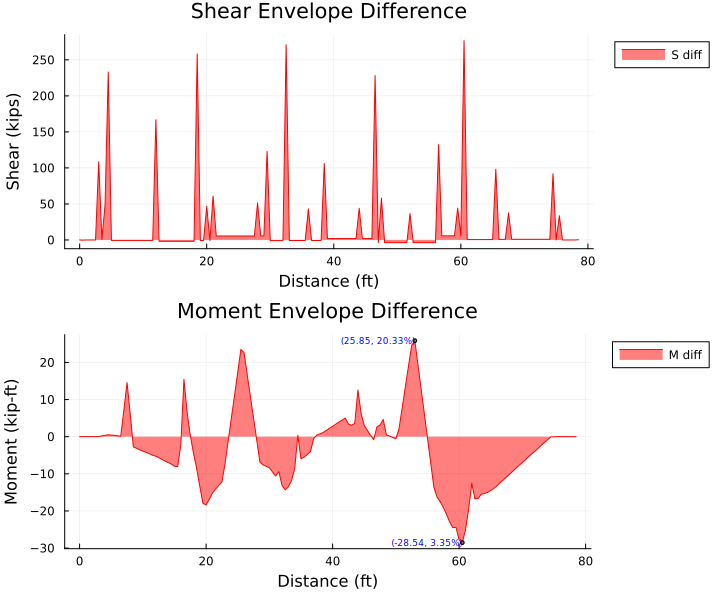
\includegraphics{03_six_col_bent_bk_files/mediabag/03_six_col_bent_bk_files/figure-pdf/cell-30-output-1.pdf}

}

\caption{Comparison: Service Shear and Moment Min Envelope Difference}

\end{figure}%

\newpage{}

\subsubsection{Live Load Comparison
(SRV)}\label{live-load-comparison-srv}

The figures below compare the working stress results for the maximum
stress envelope of the live load between the two programs. The areas in
red highlight where larsa results were greater in magnitude than the
cap18 results. There are some visible red areas in the shear diagram.
However, some of the differences can be explained by the difference in
point load modeling between the two programs. The other shear areas
where larsa results look to be higher in magnitude could potentially be
explained by the difference in how the programs run the live load. The
Larsa modeling of the live load is a little limited and conservative
methods were used.

The maximum moment values are shown to be very similar. In areas of
maximum moment, the results are within 3\%.

\begin{figure}[H]

{\centering 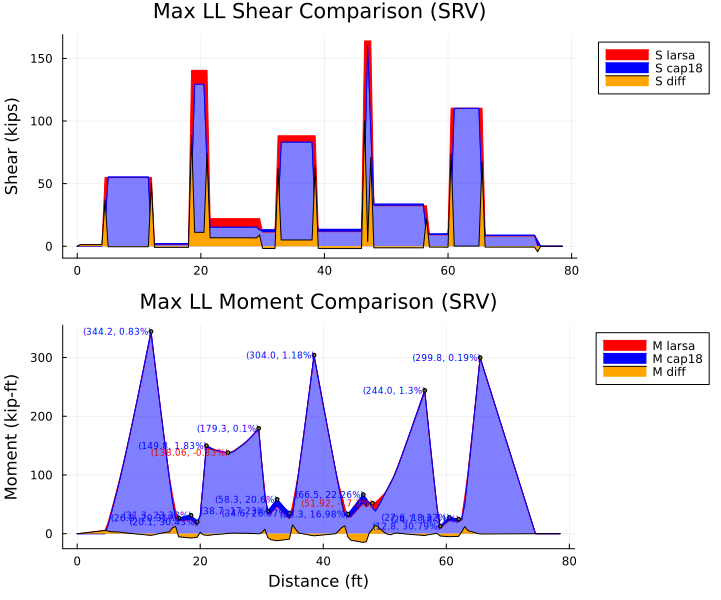
\includegraphics{03_six_col_bent_bk_files/mediabag/03_six_col_bent_bk_files/figure-pdf/cell-31-output-1.pdf}

}

\caption{Comparison: Service Shear and Moment Max LL Envelope Diagrams}

\end{figure}%

\newpage{}

The figures below compare the working stress results for the minimum
stress envelope of the live load between the two programs. The areas in
red (not the light red areas) highlight where larsa results were greater
in magnitude than the cap18 results. There are some visible red areas in
the shear diagram. However, these can be explained by the difference in
point load modeling between the two programs. There are also large red
spikes in the shear diagram for the larsa results. This is also a sign
there are some unrealistic modeling behaviors in the larsa model.

The maximum moment values are shown to be very similar. In areas of
maximum moment, the results are within 5\%.

\begin{figure}[H]

{\centering 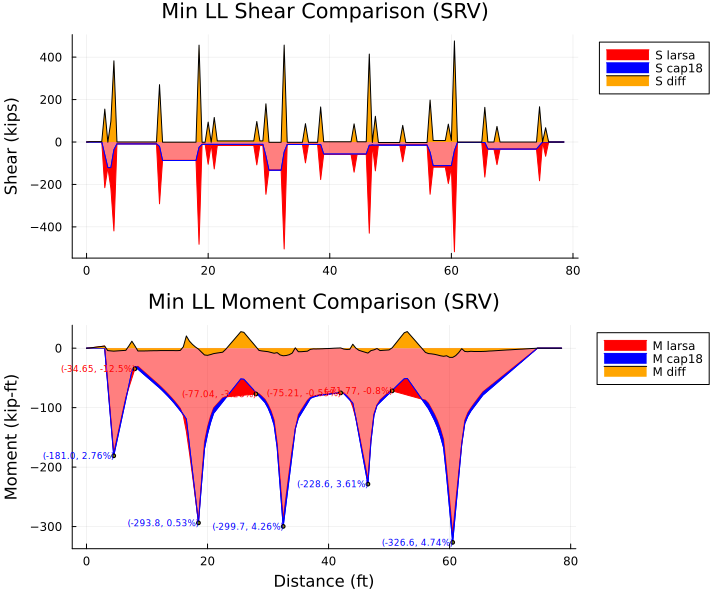
\includegraphics{03_six_col_bent_bk_files/mediabag/03_six_col_bent_bk_files/figure-pdf/cell-32-output-1.pdf}

}

\caption{Comparison: Service Shear and Moment Min LL Envelope Diagrams}

\end{figure}%

\newpage{}

\subsubsection{Maximum Support Reactions
(SRV)}\label{maximum-support-reactions-srv-2}

The figure below compares the working stress results for the maximum and
minimum reactions between the two programs. The results between programs
are within 1\% of eachother.

\begin{figure}[H]

{\centering 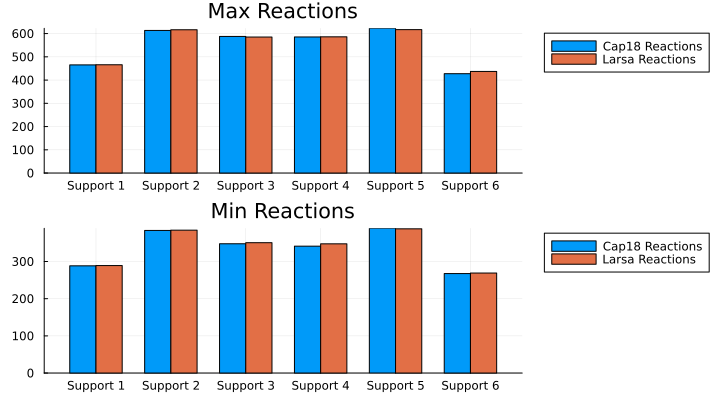
\includegraphics{03_six_col_bent_bk_files/mediabag/03_six_col_bent_bk_files/figure-pdf/cell-33-output-1.pdf}

}

\caption{Comparison: Service Reactions}

\end{figure}%

\newpage{}

\subsection{STR}\label{str-2}

\subsubsection{Envelopes of Maximum Values
(STR)}\label{envelopes-of-maximum-values-str-2}

The figures below compare the load factor results for the maximum stress
envelope between the two programs. The areas in red highlight where
larsa results were greater in magnitude than the cap18 results. There
are some visible red areas in the shear diagram. However, these can be
explained by the difference in point load modeling between the two
programs. The maximum values are shown to be very similar. In areas of
maximum moment, the results are within 3\%.

\begin{figure}[H]

{\centering 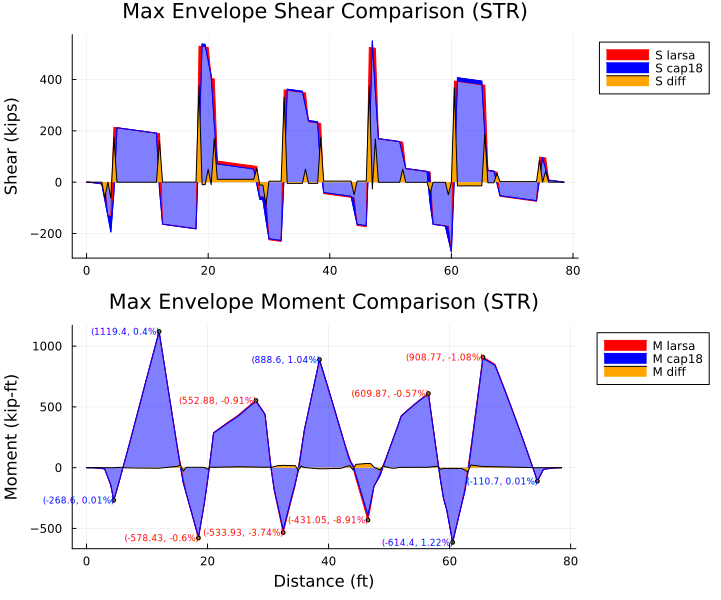
\includegraphics{03_six_col_bent_bk_files/mediabag/03_six_col_bent_bk_files/figure-pdf/cell-34-output-1.pdf}

}

\caption{Comparison: Strength Shear and Moment Max Envelope Diagrams}

\end{figure}%

\begin{figure}[H]

{\centering 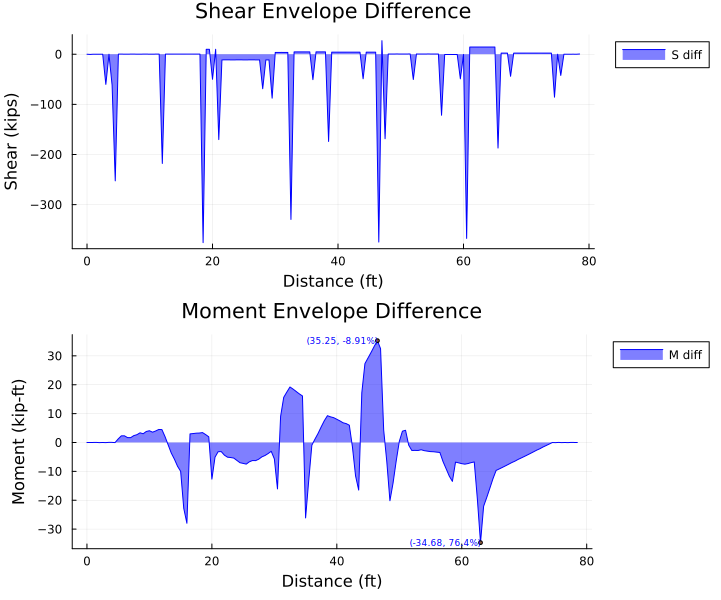
\includegraphics{03_six_col_bent_bk_files/mediabag/03_six_col_bent_bk_files/figure-pdf/cell-35-output-1.pdf}

}

\caption{Comparison: Strength Shear and Moment Max Envelope Difference}

\end{figure}%

\newpage{}

The figures below compare the load factor results for the minimum stress
envelope between the two programs. The areas in red (not the light red
areas) highlight where larsa results were greater in magnitude than the
cap18 results. There are some visible red areas in the shear diagram.
However, these can be explained by the difference in point load modeling
between the two programs. . In areas of maximum moment and shears, the
results are within 8\%. Areas where larsa results are greater than cap18
are within 5\% (these areas are also positive moments when negative
moment are being maximized).

\begin{figure}[H]

{\centering 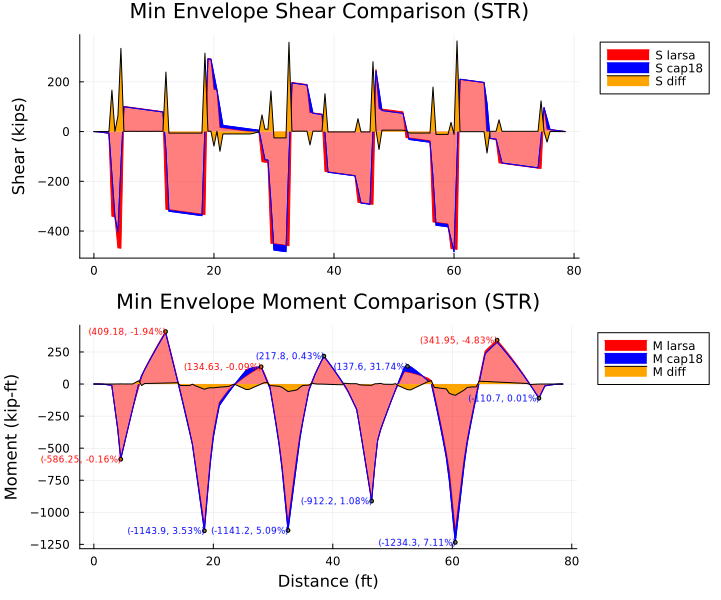
\includegraphics{03_six_col_bent_bk_files/mediabag/03_six_col_bent_bk_files/figure-pdf/cell-36-output-1.pdf}

}

\caption{Comparison: Strength Shear and Moment Min LL Envelope Diagrams}

\end{figure}%

\begin{figure}[H]

{\centering 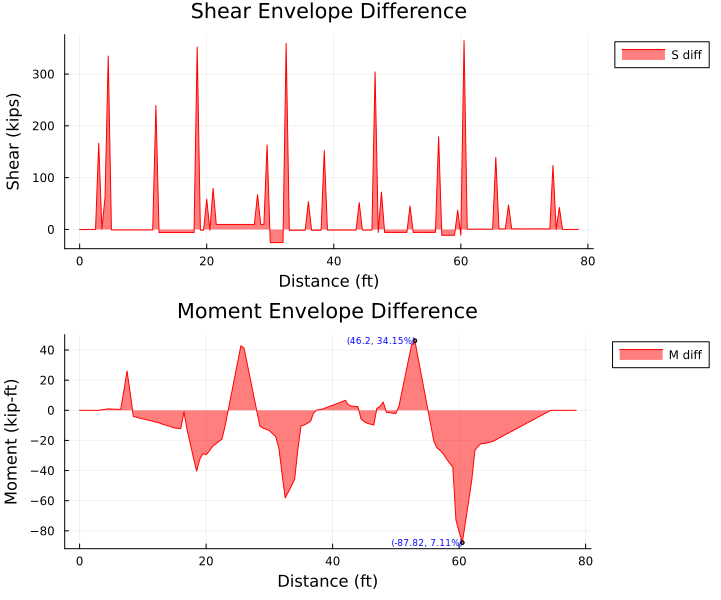
\includegraphics{03_six_col_bent_bk_files/mediabag/03_six_col_bent_bk_files/figure-pdf/cell-37-output-1.pdf}

}

\caption{Comparison: Strength Shear and Moment Min Envelope Difference}

\end{figure}%

\newpage{}

\subsubsection{Live Load Comparison
(STR)}\label{live-load-comparison-str}

The figures below compare the load factor results for the maximum stress
envelope of the live load between the two programs. The areas in red
highlight where larsa results were greater in magnitude than the cap18
results. There are some visible red areas in the shear diagram. However,
these can be explained by the difference in point load modeling between
the two programs. The maximum values are shown to be very similar. In
areas of maximum moment, the results are within 3\% (when looking at the
positive moments).

\begin{figure}[H]

{\centering 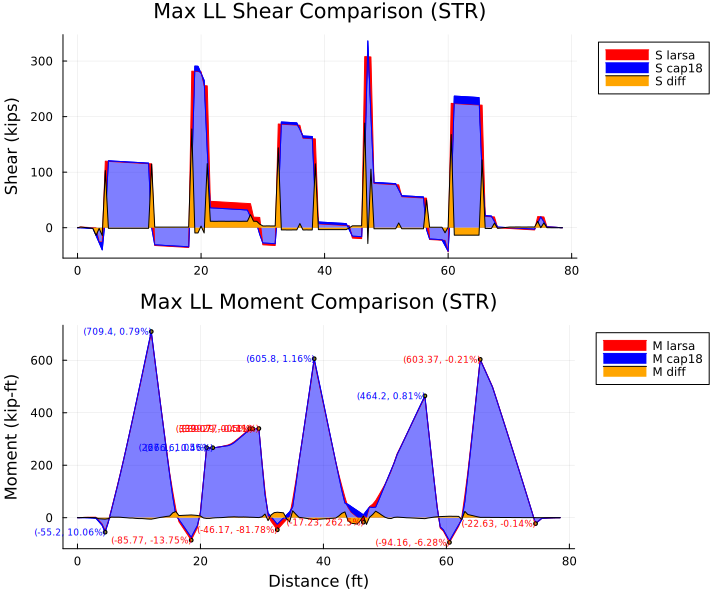
\includegraphics{03_six_col_bent_bk_files/mediabag/03_six_col_bent_bk_files/figure-pdf/cell-38-output-1.pdf}

}

\caption{Comparison: Strength Shear and Moment Max LL Envelope Diagrams}

\end{figure}%

\newpage{}

The figures below compare the load factor results for the minimum stress
envelope of the live load between the two programs. The areas in red
(not the light red areas) highlight where larsa results were greater in
magnitude than the cap18 results. There are some visible red areas in
the shear diagram. However, these can be explained by the difference in
point load modeling between the two programs. There are also large red
spikes in the shear diagram for the larsa results. This is also a sign
there are some unrealistic modeling behaviors in the larsa model.

The maximum moment values are shown to be very similar. In areas of
maximum moment, the results are greater at 11\%. However, with the
limitations of the larsa model, this is not alarming. Cap18 results are
higher and the program is doing a better job at maximizing the
controlling areas.

\begin{figure}[H]

{\centering \includegraphics{03_six_col_bent_bk_files/mediabag/03_six_col_bent_bk_files/figure-pdf/cell-39-output-1.pdf}

}

\caption{Comparison: Strength Shear and Moment Min LL Envelope Diagrams}

\end{figure}%

\newpage{}

\subsubsection{Maximum Support Reactions
(STR)}\label{maximum-support-reactions-str-2}

The figure below compares the load factor results for the maximum and
minimum reactions between the two programs. The results between programs
are within 5\% of eachother.

\begin{figure}[H]

{\centering \includegraphics{03_six_col_bent_bk_files/mediabag/03_six_col_bent_bk_files/figure-pdf/cell-40-output-1.pdf}

}

\caption{Comparison: Strength Reactions}

\end{figure}%



\end{document}
